\section{Описание практической части}
\label{sec:Chapter4} \index{Chapter4}

В нашей практической части исследования мы столкнулись с необходимостью внедрения объединённых типов в существующий
проект по разработке статически типизированного языка программирования MyTS\@.
Развитие статически типизированных языков программирования продолжает оставаться актуальной темой, поскольку такие
языки предлагают ряд преимуществ, таких как повышение надёжности и обеспечение более строгой документации кода.
При разработке статически типизированных языков программирования одним из ключевых аспектов является поддержка
различных типов данных и их комбинаций.
Объединённые типы предоставляют механизм для определения переменных, которые могут содержать значения различных типов.
Это позволяет программистам более гибко и эффективно работать с данными в коде, обеспечивая при этом строгую типизацию
и избегая возможных ошибок времени выполнения.

В данном проекте нам требовалось внедрить поддержку объединённых типов для расширения возможностей системы типов языка
программирования.
В предыдущей главе мы исследовали различные сценарии использования типов объединения в нашем языке, изучили внутреннее
устройство компилятора, а также необходимые сторонние механизмы (такие как boxing/unboxing операции и инструкции
загрузки по имени), которые потребуются нам для реализации решения.

На верхнем уровне нам необходимо внедрить наше решение в парсер (синтаксический анализатор), механизм проверки типов и
кодогенерации.
При необходимости воспользуемся отдельными проходами для модификации AST дерева.
Все ключевые алгоритмы ниже будут представлены на псевдокоде в демонстрационных целях.

\subsection{Синтаксический анализ}

Основная функция, которая парсит пришедший нам union тип, представлена следующим псевдокодом:

\begin{lstlisting}
Function ParseUnionType(FirstType):
    types = []
    types.append(FirstType)
    while NextToken() == "|":
        ReadNextToken()
        nextType = ParseTypeAnnotation()
        types.append(nextType)
    unionType = CreateUnionType(types)
    startPosition = StartPositionOfFirstType(FirstType)
    endPosition = EndPositionOfLastType(types)
    SetRangeOfUnionType(unionType, startPosition, endPosition)
    return unionType
\end{lstlisting}

Функция начинается с создания вектора типов types, который будет содержать все типы, входящие в объединённый тип.
Первый тип в объединении добавляется в вектор types.
Затем функция переходит в цикл while, который продолжается, пока текущий токен - это побитовый оператор "ИЛИ" (|).
Внутри цикла функция считывает следующий токен (переход к следующему токену).
Затем она вызывает функцию ParseTypeAnnotation, которая парсит следующий тип, на который указывает токен после
оператора "ИЛИ", и добавляет его в вектор types.
Наконец, после выхода из цикла создаётся объект unionType, представляющий объединённый тип, и инициализируется с
использованием вектора типов types.
Затем устанавливается диапазон объединённого типа от начальной позиции (локации первого типа в исходном коде)
до конечной позиции последнего типа в объединении.
Наконец, функция возвращает указатель на созданный объект unionType, который является уже частью внутреннего
представления программы.

\subsection{Анализатор типов}

Проверка типов является одним из основных этапов компилятора и происходит после создания синтаксического анализа и
построения AST дерева.
В анализаторе типов представлены главные структуры промежуточного представления для всех узлов дерева и типов
переменных.
Нам необходимо написать свой класс для union типа с необходимым функционалом для анализа и дальнейшей кодогенерации.
Этот класс должен поддерживать следующую функциональность, как и все остальные типы анализатора:

\begin{itemize}[left=2em]
    \item Отношение идентичности объединения другому типу
    \item Отношение подтипирования
    \item Отношение присвоения
    \item Отношение приведения
\end{itemize}

Кроме того, необходимо переопределить много других вспомогательных функций (например строковое представления для
вывода ошибок или ассемблерное представление для кодогенерации), а также продумать формат, в котором приходят и
обрабатываются наши компоненты объединения.

Было принято решение, что удобнее всего передавать в этот класс уже нормализованные типы, так как логически
нормализация должна происходить сразу при создании объединения.
Также после нормализации в конструкторе класса будет вычисляться низкоуровневое представление union типа, которое
впоследствии будет использоваться в среде исполнения.
Для качественной и честной кодогенерации представлять объединение на уровне байт-кода было бы правильным подходом.
Однако ввиду срочности производственной задачи было принято решение реализовать более простой вариант низкоуровневого
представления, а именно с помощью наименьшей верхней границы.
Дадим ее определение.

\subsubsection{Hаименьшая верхняя граница}

Понятие наименьшей верхней границы (LUB - least upper bound) используется там, где необходимо найти единственный тип,
который является общим супертипом для набора ссылочных типов.
Слово "наименьший" означает, что необходимо найти наиболее специфичный супертип, и не существует другого общего
супертипа, который был бы подтипом LUB\@.
Отдельный тип является наименьшей верхней границей сам по себе.
В наборе \hl{($A_1$,. . . , $A_n$)}, который содержит по меньшей мере два типа, LUB определяется следующим образом:

\begin{itemize}[left=2em]
    \item Для каждого типа в наборе определяется свой набор супертипов $SupA_i$;
    \item Вычисляется пересечение наборов $SupA_i$.
    Пересечение всегда содержит объект и, следовательно, не может быть пустым.
    \item Из пересечения выбирается наиболее специфичный тип.
\end{itemize}

Ошибка времени компиляции возникает, если какие-либо типы в исходном наборе \hl{($A_1$,. . . , $A_n$)}
не являются ссылочными типами.

\subsubsection{Алгоритм подсчета низкоуровневого представления объединения}

Низкоуровневое представление объединения необходимо для кодирования union типов в байт-код и вычисляется в основном
с использованием наименьшей верхней границы.

\begin{lstlisting}[label={lst:computelub}]
Function ComputeLowLvlType(unionType):
    preciseType = GetPreciseType(unionType)
    If preciseType is not UnionType:
        return preciseType
    lub = null
    For each type in unionType.ConstituentTypes():
        If type is NullType or lub == type:
            continue
        If lub is null:
            lub = type
            continue
        If type is ObjectType and lub is ObjectType:
            lub = GetLUB(lub.AsObjectType(), type.AsObjectType())
        Else If type is PrimitiveType:
            If lub is ObjectType:
                lub = GetLUB(lub.AsObjectType(), ConvertToObjectType(type))
            Else If lub is PrimitiveType:
                lub = LargestPrimitive(type, lub)
            Else:
                return GetGlobalObjectType()
        Else:
            return GetGlobalObjectType()
    return GetNonConstantType(lub)
\end{lstlisting}

Низкоуровневое представление может являться как ссылочным типом, так и примитивным.
Это было сделано для оптимизации объединений, содержащих литеральные типы, и будет описано подробнее в последующих
разделах.

Итак, выше на псевдокоде приведена функция вычисления нашего представления объединения и ее можно описать следующим
образом:
\begin{itemize}[left=2em]
    \item Сначала определяется наиболее точный тип для объединения.
    Наиболее точный тип определяется либо самим типом объединения, либо ограничением на типовой параметр.
    Если этот тип не является union типом, он возвращается как есть
    \item Далее инициализируется переменная lub (наименьшая общая верхняя граница) как null
    \item После чего мы входим в цикл, который перебирает все составляющие типы объединения
    \item Если текущий тип является NullType или равен lub, то он пропускается
    \item Если lub еще не установлен, он инициализируется текущим типом и продолжается следующая итерация
    \item Если оба типа (текущий и lub) являются ObjectType, определяется их наименьшая общая верхняя граница с
    помощью функции GetLUB\@.
    \item Если текущий тип является PrimitiveType, выполняются дальнейшие проверки:
    \begin{itemize}[left=2em]
        \item Если lub является ObjectType, определяется наименьшая общая верхняя граница между lub (как ObjectType) и
        текущим типом, преобразованным в ObjectType.
        \item Если lub также является PrimitiveType, вызывается функция LargestPrimitive для определения наибольшего
        примитивного типа между текущим типом и lub.
        \item В противном случае, возвращается глобальный объектный тип.
    \end{itemize}
    \item Если текущий тип не соответствует ни одному из вышеуказанных условий, возвращается глобальный объектный тип
    \item В конце, возвращается не константный тип, который является наименьшей общей верхней границей для всех
    составляющих типов union.
\end{itemize}
Возвращается именно не константное значение, потому что на уровне байт-кода нет представления для литералов.
Также низкоуровневое представление будет потом участвовать в кодогенерации и проходах по модификации AST дерева,
как примитивный тип.

\subsubsection{Алгоритм нормализации объединения}

Процесс нормализации объединения происходит в самом начале даже перед подсчетом низкоуровневого представления.
Ввиду сложности, рассмотрим алгоритм нормализации в несколько этапов, постепенно погружаясь во все более вложенные
функции.

Дадим определение нескольких небольших функций, участвующих в алгоритме:

\begin{itemize}[left=2em]
    \item Функция IsNumericUnion, определяющая, что union тип является числовым, возвращает истину в том случае, если все
составляющие типы объединения являются маленькими (unboxed) числовыми типами или числовыми литералами.
В противном случае функция возвращает ложь.
    \item Функция BoxTypes, как видно из названия, преобразует все компоненты объединения в большие (boxed) типы.
    \item Функция TryAbsorbType пытается слить воедино два типа, которые в нее пришли.
    Делает она это путем вызова функции подтипирования для обоих типов, а также довольно непростого анализа удаления
    литеральных типов, который будет описан чуть позже.
\end{itemize}

Далее опишем алгоритм линеаризации и удаления идентичных типов на псевдокоде:

\begin{lstlisting}[label={lst:normalization}]
    initialSize = len(types)
    for i from 0 to initialSize - 1:
        currentType = types[i]
        if currentType is UnionType:
            otherTypes = currentType.ConstituentTypes()
            add otherTypes to types
            types[i] = null
        else if currentType is NeverType:
            types[i] = null
    EliminateAllNullTypes(types)
    if not IsNumericUnion(types):
        BoxTypes(types)
    for each cmp in types:
        for each it from cmp + 1 to end of types:
            merged = TryAbsorbType(cmp, it)
            if merged is not null:
                if merged == cmp:
                    remove it from types
                else:
                    remove cmp from types
                    cmp = next element after cmp
            else:
                continue to next it
\end{lstlisting}

В результате работы этого алгоритма получается более оптимизированный и компактный union тип, который может
использоваться в дальнейших вычислениях и проверках типов.
Опишем подробнее, какие шаги присутствуют в написанном коде:

\begin{itemize}[left=2em]
    \item Линеаризация: Развертывание всех вложенных union типов и удаление типов never.
    Для каждого элемента в списке types:
    \begin{itemize}[left=2em]
        \item Если элемент является union типом, его составляющие типы добавляются в конец списка types.
        \item Если элемент является типом never, он помечается как null.
    \end{itemize}
    Стоит отметить, что рекурсивно раскрываются все вложенные объединения, так как если union тип попал в алгоритм
    нормализации, значит он был уже кем-то создан.
    А как известно еще перед созданием объединения все типы, которые в него поступают, проходят такой же процесс линеаризации.

    \item Далее удаляются все null элементы из списка types, которые были помечены ранее.
    Также размер списка types уменьшается до количества всех не null элементов.
    \item Boxing типов: Если union не состоит из числовых типов, вызывается функция BoxTypes, описанная ранее.
    \item Слияние подтипов: Итерация по каждому элементу в списке types.
    Для каждого элемента проверяются все последующие элементы на возможность слияния с помощью функции TryAbsorbType.
    Если два элемента могут быть объединены, выполняется их слияние:
    \begin{itemize}[left=2em]
        \item Если слияние возвращает первый элемент, второй элемент удаляется.
        \item Если слияние возвращает второй элемент, первый элемент удаляется, и текущая итерация смещается на
        следующий элемент после текущего.
    \end{itemize}
\end{itemize}

В более подробном объяснении нуждается процесс слияния литеральных типов, поскольку спецификацией задается требование,
что любое значение литерала, попадающее в более расширенный числовой тип, удаляется из объединения.
На практике для каждого примитивного типа у нас существует отдельный класс для анализатора типов со своими отношениями
подтипирования и идентичности.
В этих отношениях в рамках одного примитивного класса невозможно обрабатывать все другие примитивные классы из-за
громоздкости и возможных конфликтов с другими компонентами анализатора.
Поскольку данные правила подтипирования и удаления литералов задействованы только в объединениях, то логично реализовать
необходимый функционал на месте и сделать его частью класса анализатора union.

Следующий псевдокод описывает алгоритм проверки, может ли константный литерал быть присвоен целевому типу в union типе.
Алгоритм включает несколько этапов: проверку типов константы и целевого типа, проверку идентичности типов и проверку
соответствия константы целевому типу:

\begin{lstlisting}[label={lst:literalassignable}]
Function IsLiteralAssignableTo(literal, target):
    if target == GlobalObjectType:
        return true
    if literal is StringType:
        return target is StringType and
                (not target is LiteralType or IsIdentical(literal, target))
    if literal is BigIntType:
        return target is BigIntType and
                (not target is LiteralType or IsIdentical(literal, target))
    if not target is PrimitiveType:
        if target is UnboxableObject:
            target = ToPrimitiveType(target)
        else:
            return false
    return IsIdentical(literal, target) or IsLiteralFitsToType(literal, target)
\end{lstlisting}
Опишем шаги из псевдокода подробнее:

\begin{itemize}[left=2em]
    \item Если target является глобальным объектным типом, возвращается true, так Object является доминирующим типом
    над любой компонентой объединения. 
    \item Обработка строковых литералов: Если literal имеет тип StringType, проверяется, что target тоже является 
    строковым типом и либо не является константным, либо идентичен literal. 
    \item Обработка типов BigInt: Если literal имеет тип BigIntType, проверяется, что target тоже является типом
    BigInt и либо не является константным, либо идентичен literal. 
    \item Далее происходит обработка большого (boxed) целевого типа:
    если target не является примитивным типом, значит он является объектом.
    Для случая объекта проверяется, является ли target большим типом.
    Если да, то target заменяется примитивным встроенным типом, полученным с помощью функции ToPrimitiveType.
    Если нет, возвращается false. 
    \item В итоге возвращается результат проверки идентичности literal и target на уровне классов анализатора или
    результат соответствия литерала целевому типу с помощью функции IsLiteralFitsToType
\end{itemize}

Стоит упомянуть принцип работы функции IsLiteralFitsToType.
Она берет значение литерала и напрямую сравнивает его с наименьшим и наибольшим значением target типа, используя функцию
стандартной библиотеки C++ std::numeric\_limits.

\subsubsection{Алгоритм отношения идентичности объединения другому типу}

Отношение идентичности определяет с каким другим объектом или типом наше объединение можно считать абсолютно идентичными.
Отношение идентичности для ссылочных типов означает, что у этих объектов одни и те же супертипы, один и тот же узел
AST дерева, задающий определение типа объекта, а также один и тот же набор типовых параметров и флагов.
Отношение идентичности для примитивных типов определяется равенством классов анализаторов (то есть и тот и другой
примитивный тип выражаются через IntType, например), а также равенством значений, если этот класс представляет собой
константу.

Для объединения был реализован свой алгоритм определения отношения идентичности, который можно разбить на две части:
идентичность в случае числового объединения и идентичность для объединения ссылочного типа.
Рассмотрим алгоритм, написанный на псевдокоде:

\begin{lstlisting}
Function Identical(thisType, otherType):
    if otherType is UnionType:
        if EachTypeIdenticalToSomeType(thisType, otherType) and
           EachTypeIdenticalToSomeType(otherType, thisType):
            return true
    if thisType.IsNumericUnion() and otherType is PrimitiveType:
        return Identical(thisType.lowLvlType, otherType)
    return false
\end{lstlisting}
Здесь thisType это наш тип объединения, который мы хотим проверить на идентичность другому типу.
Рассмотрим реализованные шаги подробнее:
\begin{itemize}
    \item Если otherType также является объединением, проверяется, что каждый тип в текущем union типе связан с
    каким-то типом в otherType и наоборот.
    Функция EachTypeIdenticalToSomeType используется для проверки этой связи.
    Если обе проверки выполняются, то типы считаются идентичными.
    \item Если текущий тип (thisType) является числовым union типом и otherType является примитивным типом
    (PrimitiveType), проверяется их идентичность с помощью низкоуровневого представления lowLvlType.

    lowLvlType подсчитывается при создании объединения, как было описано ранее.
    \item Если ни одно из условий не выполняется, возвращается результат отношения false.
\end{itemize}
Сравнение с низкоуровневым представлением вместо самого объединения связано с тем, что отношение идентичности для
примитивных типов и литералов слишком строгое и нам важно только то, каким типом будет являться наш union по факту
при кодировании в байт-код.

\subsubsection{Алгоритм отношения подтипирования}

Отношение подтипирования, как видно из названия, определяет, является ли один тип супертипом другого.
Для ссылочных типов рекурсивно проверяется, выполняется ли отношение идентичности между каким-либо супертипом другого
объекта и рассматриваемым ссылочным типом.
Подтипирование также выполняется и для идентичных типов.
Таким образом, отношение идентичности самое сильное из отношений, которое учитывается во всех остальных алгоритмах
отношений.
Для объединения был реализован свой метод, определяющий отношение подтипирования и заключается он в том, что
все компоненты union типа обходятся по порядку.
Для каждой составляющей объединения вызывается метод отношения IsSuperType(ct, other), где ct - это компонента union, а
other - потенциальный подтип.
В результате получается худющие правила подтипирования:
\begin{itemize}
    \item Объединение, состоящее из компонент \hl{($A_1$,. . . , $A_n$)} является подтипов другого объединения, состоящего
    из компонент \hl{($B_1$,. . . , $B_k$)}, если для каждого $B_i$ выполняется отношение подтипирования с $A_j$, то
    есть функция \hl{IsSuperType($A_j$, $B_i$)} возвращает истину для любых i и j.
    \item В частном порядке для объединений, состоящих из литеральных типов, следует, что отношение подтипирование
    возвращает истину только в том случае, если все литеральные типы одного объединения идентичны без явного
    приведения типов каким-либо компонентам из другого объединения.
\end{itemize}
Например, объединение \hl{1|2} является подтипом объединения \hl{1|2|3}, но не является подтипом объединения \hl{1|4},
так как для литералов 2 и 4 не выполняется отношение идентичности.

\subsubsection{Алгоритм отношения присвоения}

Отношение присвоения определяет, может ли какой-то тип быть присвоен объединению или наоборот.
Здесь могут учитываться контекст и неявные преобразования.

Функция RelationTarget является основной частью алгоритма и определяет, может ли источник (source) быть присвоен целевому
типу (this union type) в контексте отношений типов.
Это выполняется путем проверки, относится ли источник к одному из составляющих типов объединения.
Также учитывается необходимость применения boxing/unboxing преобразований.
Рассмотрим псевдокод этой функции:

\begin{lstlisting}[label={lst:relationtarget}]
Function RelationTarget(source):
    boxedSource = BoxType(source)
    if boxedSource != source and not ApplyBoxing():
        return false
    for each ct in ConstituentTypes:
        if IsAssignable(boxedSource, ct):
            if boxedSource != source:
                node.SetBoxingFlag(boxedSource)
            return true
    if boxedSource == source:
        return IsSupertype(thisUnion, boxedSource)
    related = false
    for each ct in ConstituentTypes:
        if IsAssignable(source, BoxType(ct)):
            if not IsNumericUnion():
                node.SetBoxingFlag(ct)
            related = true
    return related
\end{lstlisting}

Алгоритм может быть разбит на следующие шаги:

\begin{itemize}[left=2em]
    \item BoxType(source): Упаковываем тип источника, преобразуя его в соответствующий объектный тип
    (например, int к Integer).
    \item Если большой тип отличается от исходного и не требуется применять boxing, функция завершает выполнение.
    \item Далее проходим по всем типам, составляющим объединение и проверяем отношение присвоения boxed источника
    текущему типу из union.
    Если присвоение возможно, устанавливаем флаг boxing (если нужно) и возвращаем true.
    \item Если boxed источник совпадает с исходным, проверяем, является ли текущий union тип супертипом для источника.
    \item Далее инициализируем переменную related как false и проходим по всем типам, составляющим union.
    \item Внутри цикла проверяем, можно ли присвоить исходный источник текущему типу из union после упаковки.
    Если присвоение возможно, устанавливаем флаг boxing (если union тип не числовой) и устанавливаем related как true.
    \item В конечном счете возвращаем значение переменной related, указывающее на возможность присвоения.
\end{itemize}

Эта функция будет позже повторно использована для отношения приведения, так как это понятие очень близко к отношению
присвоения.
В результате она вызывается из другой функции присвоения, которая переопределяется для всех классов анализтора и
называется IsAssignable.

\subsubsection{Алгоритм отношения приведения}

Отношение приведения определяет, может ли наше объединение быть преобразовано в какой-либо другой тип с помощью
явного приведения.
В данной инфраструктуре компилятора, для каждого класса анализатора необходимо переопределить два метода приведения:
Cast и CastT\@.
Функция Cast определяет, можно ли явно привести рассматриваемый класс анализатора к какому-либо другой типу.
В свою очередь CastT действует наоборот и возвращает истину, если какой-либо другой тип может быть явно приведен
текущему классу анализатора.

Реализуем данные методы и отобразим их на языке псевдокода:

\begin{lstlisting}[label={lst:casttarget}]
Function Cast(target):
    If target is PrimitiveType:
        If not ApplyUnboxing():
            return false
        node.SetUnboxingFlag(target)
    If InCastingContext():
        For each ct in ConstituentTypes:
            If IsCastable(ct, target):
                return true
        return false
    If IsNumericUnion():
        return IsCastable(thisUnion.lowLvlType, target)
    res = true
    For each ct in ConstituentTypes:
        If not IsCastable(ct, target):
            res = false
            break
    return res
\end{lstlisting}

Этот метод описывает возможность приведения union типа к целевому типу.
Вот что происходит на каждом этапе:

\begin{itemize}[left=2em]
    \item Если целевой тип (target) является примитивным (PrimitiveType), проверяется возможность применения unboxing.
    Если unboxing невозможен (not ApplyUnboxing()), функция возвращает false.
    В противном случае устанавливается соответствующий флаг unboxing для узла AST дерева (node.SetUnboxingFlag(target)).
    \item Если функция вызвана в контексте приведения (InCastingContext()), проверяется возможность приведения
    каждой компоненты объединения (ct) к целевому типу (target).
    Если хотя бы один тип из составляющих типов union (ConstituentTypes) приводим к целевому типу, функция возвращает true.
    Если ни один из типов не приводим, функция возвращает false.
    \item Если union тип является числовым, проверяется возможность приведения его низкоуровневого представления к
    целевому типу.
    \item Если union тип не является числовым, проверяется возможность приведения каждой компоненты объединения
    к целевому типу.
    Если хотя бы одна компонента не приводима к target, то переменная res устанавливается в false и цикл прерывается.
    В конце функция возвращает значение res.
\end{itemize}

Пример использования:
предположим, что у нас есть union тип A | B | C, где A, B и C — это различные типы.
Нам нужно определить, может ли этот union тип быть приведен к другому типу T.
Функция Cast выполняет эту проверку, следуя описанным шагам, и возвращает true, если приведение возможно, и
false в противном случае.

Метод CastTarget работает точно таким же образом, что и Assignable, и вызывается внутри себя ту же функцию RelationTarget,
которая была описана ранее.
Единственная разница заключается в предикате для функции RelationTarget - в случае отношения присвоения этот предикат
проверяет Assignable каждой компоненты, а в случае отношения приведения - IsCastable.

\subsection{Кодогенерация объединений}

В данном разделе будут описаны алгоритмы кодогенерации для объединений, а также различные реализованные
проходы компилятора, которые позволяют модифицировать AST дерево и подготовить его к дальнейшим преобразованиям.

\subsubsection{Алгоритм понижающей трансформации доступа к полю}

В данной секции будет описан алгоритм, позволяющий сгенерировать необходимые сущности в байт-код для доступа к полям
объединения.
Как было сказано в главе исследования и построения решения задачи, нам необходимо воспользоваться готовыми инструкциями
загрузки и выгрузки значения поля любого объекта по имени - LON\_INST и SON\_INST\@.
Для того, чтобы ими воспользоваться также нужно создать синтетический класс и записать в него информацию об имени поля
и его типе.

Однако, прежде чем перейти к описанию понижающей трансформации, стоит упомянуть, что на этапе анализатора типов нам
нужно удостовериться, что запрашиваемый доступ к полю валиден.
Для этого необходимо:
\begin{itemize}[left=2em]
    \item Пройтись по всем компонентам объединения
    \item Для каждой компоненты проверить, существует ли запрашиваемое поле в списке свойств объекта
    \item Проверить, что тип данного поля во всех компонентах одинаков, иначе выдать ошибку компиляции
    \item Установить низкоуровневое представление объединения в качестве типа всего выражения доступа к полю (ранее им
    был непосредственно union тип)
\end{itemize}
В случае, если проверка прошла успешно, мы доходим до этапа понижающей трансформации.

На следующем этапе реализуется создание и управление синтетическими классами и их свойствами для union типов.
Основные действия происходят в трёх функциях.
Вот их описание на псевдокоде:

\begin{lstlisting}[label={lst:getUnionFieldClass}]
Function GetUnionMemberAccessClass():
    foundVar = SearchClassInScope(unionMemberAccessClassName)
    If foundVar != null:
        return foundVar
    ident = CreateIdentNode(unionMemberAccessClassName)
    decl, var = CreateVarDecl(ident)
    classDef = CreateClassDefinition(ident, GLOBAL)
    classDef.SetScope(GetScope())
    classDecl = CreateClassDeclaration(classDef)
    classDef.SetType(GlobalObjectType())
    var.SetScope(classDef.Scope())
    return classDef
\end{lstlisting}

Данный псевдокод описывает функцию GetUnionMemberAccessClass, которая предназначена для поиска или создания
специального синтетического класса, используемого для доступа к членам union типов.
Вот описание шагов, что выполняет этот псевдокод:

\begin{itemize}[left=2em]
    \item Поиск существующего класса: в глобальной области видимости (scope) ищется класс с именем
    unionMemberAccessClassName.
    Если такой класс найден (foundVar не null), он возвращается.
    \item Создание нового класса: если нет, то создаётся новый узел идентификатора (ident) с именем unionMemberAccessClassName.
    Далее создаются новое объявление переменной, привязанное к идентификатору, а также новое объявление и определение класса
    с указанным идентификатором и глобальным модификатором (GLOBAL).
    \item После чего проставляются необходимые области видимости для всех созданных сущностей
    \item Возвращается определение созданного класса.
\end{itemize}

Далее рассмотрим функцию CreateUnionMemberAccessClassProperty, которая предназначена для создания или поиска свойства
в нашем синтетическом классе unionMemberAccessClass:

\begin{lstlisting}[label={lst:UnionFieldClassProperty}]
Function CreateUnionMemberAccessClassProperty(fieldType, propName):
    unionMemberAccessClass = GetUnionMemberAccessClass()
    classScope = unionMemberAccessClass.GetScope()
    foundVar = classScope.SearchProperty(propName)
    If foundVar != null:
        return foundVar
    fieldIdent = CreateIdentifierForField(propName)
    field = CreateClassPropertyNode(fieldIdent)
    field.SetType(fieldType)
    unionMemberAccessClass.AddProperties(field)
    return var.AsLocalVariable
\end{lstlisting}
Вот описание шагов, которые выполняет этот псевдокод:

\begin{itemize}[left=2em]
    \item Получение синтетического класса: вызывается функция GetUnionMemberAccessClass, описанная ранее.
    \item Далее получаем область видимости этого класса
    \item Поиск существующего свойства: в области видимости класса ищется свойство с именем propName.
    Если такое свойство найдено, оно возвращается.
    \item Создание нового свойства: создаётся новый идентификатор для свойства с именем propName.
    \item Создаёт узел поля класса с созданным идентификатором и устанавливается его тип в соответствие с fieldType.
    \item Созданное поле добавляется в синтетический класс.
\end{itemize}

Вкратце можно описать так, что если свойство уже существует, оно возвращается.
Если свойства нет, оно создаётся и добавляется в класс.
Далее из обработчика понижающей трансформации вызывается последняя функция, которая и осуществляет всю работу.
Важно отметить, что если получилось так, что у низкоуровневого представления такое свойство уже есть, то данные
инструкции для доступа по имени не генерируется и байт-код использует свойства супертипа объединения.

\subsubsection{Алгоритм понижения бинарного оператора}

На этапе компиляции нам неизвестен фактический тип значения, который может оказаться в объединении во время исполнения
программы.
Это значение может иметь как тип любой из компонент объединения, так и их подтипы.
В результате чего возникает проблема правильного считывания значения при бинарных операциях.
Бинарными операторами могут выступать сравнение ==, сложение, вычитание и прочие функции.
Вообще говоря, любые операции, кроме сравнения на равенство, запрещено делать с объединениями.
Однако в нашей работе сделано исключение для числовых union типов.
Для них остаются легальными такие операции, как сложение, сравнение на больше или меньше и прочие.

Сначала опишем понижающую трансформацию для оператора сравнения на равенство.
Забегая вперед, нам необходимо будет сгенерировать несколько statement-ов и добавить их в базовый блок, в котором находится
искомое нами бинарное выражение, содержащее объединение.
Это означает, что нам нужно обрабатывать не какое-то конкретное выражение, а целый блок.
Обозначим по какому фильтру мы будет отбирать наше бинарное выражение:

\begin{itemize}[left=2em]
    \item На этапе анализа типов, обозначаем тип бинарной операции union типом для дальнейшей обработки
    \item Если левая или правая часть бинарной операции является типом объединения, то возвращается истина.
    В противном случае возвращается ложь.
\end{itemize}
Далее для каждого отфильтрованного выражения будет запускать процесс генерации instaceOf дерева.
Он описывается следующим псевдокодом:

\begin{lstlisting}[label={lst:binaryOp}]
Function ReplaceBinaryExprInStmt(block, binaryExpression):
    statement = FindStatement(binaryExpression)
    binaryVarDecl = CreateVariableDeclaration(statement, binaryExpression)
    varDeclId = binaryVarDecl.GetFirstDeclaratorId()
    instanceofTree = null
    binaryExpression.SetLeft(CreateTmpVar(statement, binaryExpression.Left()))
    binaryExpression.SetRight(CreateTmpVar(statement, binaryExpression.Right()))
    isLeftUnion = binaryExpression.Left().IsUnionType()
    unionNode = If isLeftUnion Then binaryExpression.Left() Else binaryExpression.Right()
    For each ct in unionNode.ConstituentTypes():
        If not ct.IsUnboxable() AND not ct.IsLiteral():
            continue
        testExpr = CreateInstanceofExpression(unionNode, ct)
        If IsDuplicateBranch(instanceofTree, testExpr):
            continue
        clonedBinaryExpr = binaryExpression.Clone()
        consequentBlock = CreateAssignmentBlock(varDeclId, ProcessBinaryOperands(clonedBinaryExpr, ct))
        instanceofTree = CreateIfStatement(testExpr, consequentBlock, instanceofTree)
    statement.ReplaceBinaryExpressions(varDeclId)
    InsertAfter(statement, binaryVarDecl, instanceofTree)
    return block
\end{lstlisting}
Функция ReplaceBinaryExprInStmt является одной из двух основных логик понижающей трансформации.
Опишем ее по шагам:

\begin{itemize}[left=2em]
    \item Находим statement соответствующий бинарному выражению, чтобы определить, где оно находится в исходном коде.
    \item Создаем новое объявление переменной (binaryVarDecl) для бинарного выражения, чтобы хранить результат
    вычисления бинарного выражения.
    Получаем идентификатор первой объявленной переменной (varDeclId) для последующего использования.
    \item Заменяем левый (Left) и правый (Right) операнды бинарного выражения на временные переменные, которые
    будут использоваться для хранения промежуточных результатов.
    \item Определяем, является ли левый операнд union-типом (isLeftUnion).
    Устанавливаем unionNode как левый или правый операнд в зависимости от того, какой из них является union-типом.
    \item Проходим по всем составным типам (ConstituentTypes) объединения,
    пропуская типы, которые не являются unboxable объектами и не являются литералами.
    \item Для каждого подходящего типа создаем выражение instanceof, чтобы проверить, соответствует ли фактическое значение
    union типа какой-либо его компоненте.
    Проверяем, не является ли ветка instanceof дублирующейся, и пропускаем её, если это так.
    \item Клонируем текущее бинарное выражение для последующей обработки.
    \item Создаем блок присваивания (consequentBlock), который будет выполнен, если instanceof проверка будет успешна.
    В блоке присваивания обрабатываем операнды бинарного выражения и присваиваем результат идентификатору переменной (varDeclId).
    \item Добавляем новое if-выражение в дерево instanceofTree, чтобы включить новую проверку instanceof и
    соответствующий блок присваивания.
    \item Заменяем все вхождения бинарного выражения в исходном выражении на идентификатор новой переменной (varDeclId).
    \item Вставляем объявление переменной (binaryVarDecl) и дерево instanceofTree после исходного выражения,
    чтобы сохранить новые преобразования в коде.
    \item Возвращаем измененный блок кода (block), который теперь содержит преобразованные выражения и проверки.
\end{itemize}
Опишем другую важную функцию, участвующую в этом преобразовании - ProcessBinaryOperands.

\begin{lstlisting}[label={lst:processBinary}]
Function ProcessOperandsInBinaryExpr(expr, constituentType):
    isLhsUnion = expr.Left().IsUnionType()
    unionNode = If isLhsUnion Then expr.Left() Else expr.Right()
    otherNode = If isLhsUnion Then expr.Right() Else expr.Left()
    unionAsExpr = ProcessUnionOperand(constituentType, unionNode, otherNode.GetType())
    otherAsExpr = ProcessOtherOperand(constituentType, otherNode, otherNode.GetType())
    If isLhsUnion Then
        expr.SetLeft(unionAsExpr)
        expr.SetRight(otherAsExpr)
    Else
        expr.SetRight(unionAsExpr)
        expr.SetLeft(otherAsExpr)
    If expr.Left().IsPrimitiveType() and expr.Right().IsPrimitiveType() Then
        expr.SetOperationType(unionAsExpr.GetType())
    Else
        expr.SetOperationType(GlobalObjectType())
    expr.SetType(GlobalBooleanType())
    return expr
\end{lstlisting}
Вот, что она делает по шагам:

\begin{itemize}[left=2em]
    \item Определение, является ли левый операнд union типом.
    Это важно для того, чтобы правильно обработать объединение и другой операнд.
    \item Далее идет обработка unionNode, используя другую важную функцию ProcessUnionOperand, которая подготавливает
    тип объединения к сравнению.
    Также обработывается otherNode, используя функцию ProcessOtherOperand, которая подготавливает другой операнд к сравнению.
    \item Происходит замена левого и правого операнда в исходном выражении на обработанные выражения в зависимости от
    того, какой из операндов является union-типом.
    \item Если оба операнда являются примитивными типами, то тип операции тоже становится примитивным.
    Если хотя бы один операнд не является примитивным типом, тип операции становится GlobalObjectType.
    Это нужно для корректного сравнения value и ссылочных типов в среде исполнения.
    \item Поскольку результат сравнения всегда
    будет булевым значением, результирующий тип выражения устанавливается как GlobalBooleanType.
    \item В конце возвращается обновленное выражение, которое теперь содержит обработанные операнды и корректные типы.
\end{itemize}
Для наглядности изобразим обобщенную реализацию алгоритма на схеме:

\begin{figure}[h]
    \centering
    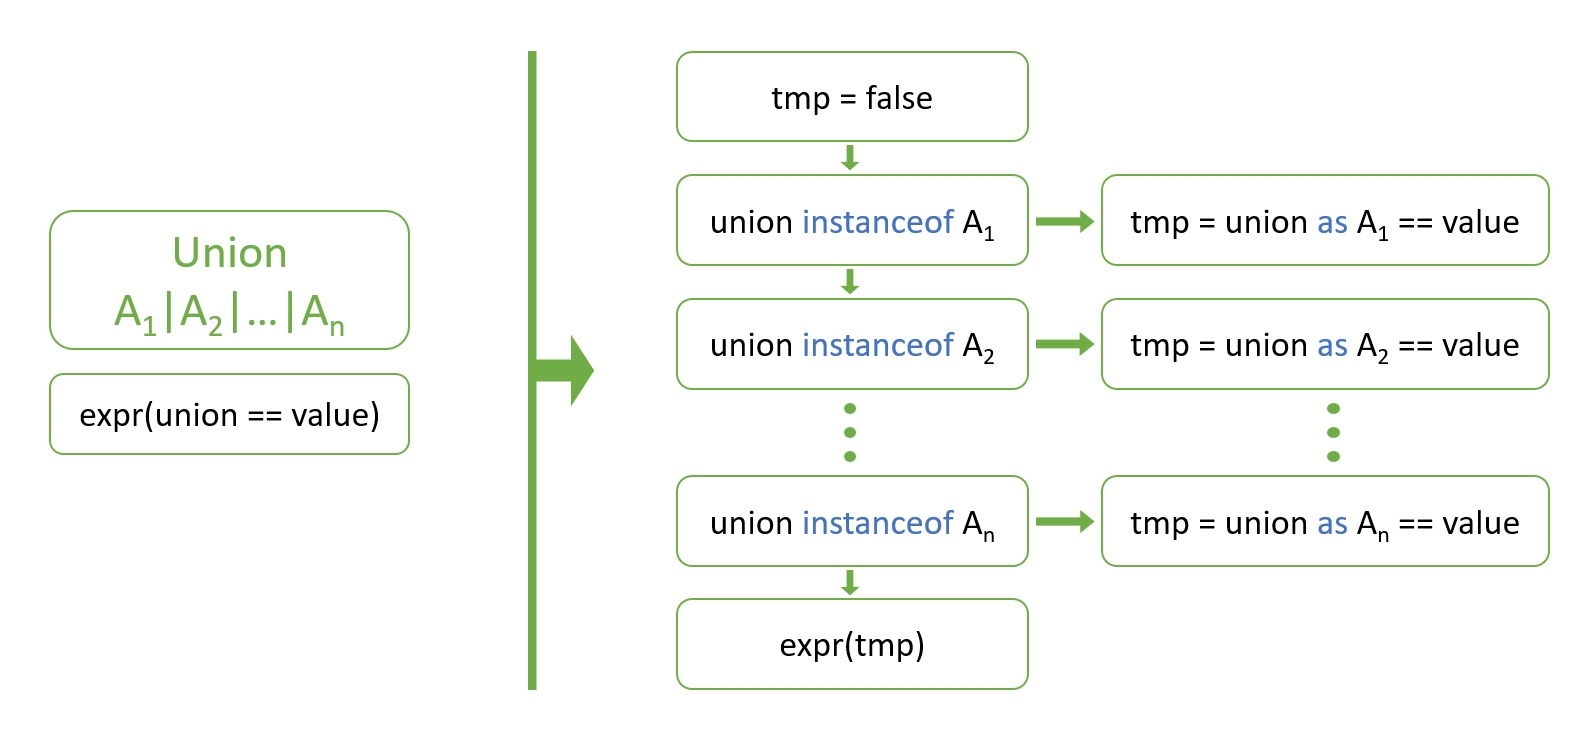
\includegraphics[scale=0.3]{binaryLowering.jpg}
    \caption{Алгоритм понижающей трансформации бинарного оператора сравнения}\label{fig:figure}
\end{figure}

Тут стоит выделить конкретнее, по какой схеме обрабатываются операнды в зависимости от их типа.

В таблице ниже описываются восемь случаев обработки операндов в выражении, где операнды могут иметь разные типы.
В таблице указаны типы операндов (cType и other) и соответствующие модификации для объединения и другого операнда
в каждом из случаев:

\begin{table}[h]
    \centering
    \begin{tabular}{|c|c|c|}
        \hline
        cType & other & преобразование \\
        \hline
        p & p & union as p; None \\
        \hline
        p & b & union as p; unbox  \\
        \hline
        b & p & union as p; None   \\
        \hline
        b & b & union as p; unbox  \\
        \hline
        p & C & union as box(p); None  \\
        \hline
        b & C & union as b; None  \\
        \hline
        C & p & union as C; box(p)  \\
        \hline
        C & b & union as C; None  \\
        \hline
    \end{tabular}
\end{table}

Обозначения:
\begin{itemize}[left=2em]
    \item cType: Тип элемента union.
    \item other: Тип другого операнда.
    \item p: Примитивный тип.
    \item b: Упакованный (boxed) тип.
    \item C: Некоторый неупаковываемый объект.
\end{itemize}
Вот описание этих случаев:
\begin{itemize}[left=2em]
    \item cType = примитивный тип (p), other = примитивный тип (p):

    union обрабатывается как примитивный тип.
    Никакие дополнительные преобразования не требуются.

    \item cType = примитивный тип (p), other = упакованный тип (b):

    union обрабатывается как примитивный тип.
    Другой операнд (other) распаковывается (unbox).

    \item cType = упакованный тип (b), other = примитивный тип (p):

    union обрабатывается как примитивный тип.
    Никакие дополнительные преобразования не требуются.

    \item cType = упакованный тип (b), other = упакованный тип (b):

    union обрабатывается как примитивный тип.
    Другой операнд (other) распаковывается (unbox).

    \item cType = примитивный тип (p), other = некоторый неупаковываемый объект (C):

    union обрабатывается как упакованный примитивный тип (box(p)).
    Никакие дополнительные преобразования не требуются.

    \item cType = упакованный тип (b), other = некоторый неупаковываемый объект (C):

    union обрабатывается как упакованный тип (b).
    Никакие дополнительные преобразования не требуются.

    \item cType = некоторый неупаковываемый объект (C), other = примитивный тип (p):

    union обрабатывается как тип (C).
    Другой операнд (other) упаковывается (box(p)).

    \item cType = некоторый неупаковываемый объект (C), other = упакованный тип (b):

    union обрабатывается как тип (C).
    Никакие дополнительные преобразования не требуются.
\end{itemize}

\subsection{Оптимизация объединений}

Использование union типов предполагает возникновение ряда проблем, связанных с производительностью и сложностью анализа
типов во время компиляции.
Для повышения эффективности и точности анализа union типов применяются различные оптимизации.
Эти оптимизации нацелены на улучшение обработки union типов путем уменьшения их сложности и упрощения работы компилятора.
Основные задачи оптимизации union типов включают:

\begin{itemize}[left=2em]
    \item Нормализация:
    Преобразование сложных union типов в линейную форму для упрощения анализа.
    Удаление дублирующихся типов внутри union, что снижает количество проверок и операций во время компиляции.

    \item Упрощение иерархии типов:
    Выявление и удаление подтипов, которые перекрываются или дублируются.
    Приведение union типов к наиболее общим формам, что позволяет компилятору выполнять оптимизации на более высоком уровне.

    \item Оптимизация операций с union типами:
    Эффективная обработка операций сравнения, присваивания и приведения типов.
    Специализация и оптимизация часто используемых операций с union типами для улучшения производительности исполняемого кода.

    \item Преобразование кода для union типов:
    Преобразование выражений и операций, включающих union типы, в более эффективные формы.
    Введение вспомогательных структур и механизмов для упрощения работы с union типами в исполняемом коде.
\end{itemize}

Оптимизации позволяют снизить количество проверок типов и преобразований во время выполнения, что непосредственно
влияет на скорость работы программы.
Также удаление дублирующих и избыточных типов уменьшает размер исходного кода и конечного бинарного файла.
Оптимизированный код с union типами становится более структурированным и понятным, что облегчает его
сопровождение и развитие.

Процесс нормализации объединений уже был описан ранее.
Основной же оптимизацией данной работы является упрощение кодогенерации для объединений, содержащих только числовые типы.
Поскольку при нормализации в отсутствие нечисловых типов все не литеральные примитивные типы сливаются в один наибольший,
единственной возможностью остаться union типом является наличие литералов среди притимвных типов объединения.
Соответственно, функция IsNumericUnion, реализованная в анализаторе типов, возвращает истину, если наше объединение
состояит только из числовых типов, причем среди них есть числовые литералы.
И возвращает ложь во всех остальных случаях.
Таким образом, в определенных случаях (чаще всего в тернарных выражениях) удается избежать использования излишних
boxing и unboxing операций, так как они являются очень дорогостоящими вызовами в среде исполнения.
Кодирование объединения в примитивный тип дает большие возможности для оптимизаций, а также для JIT и AOT исполнения.
Однако увеличивается сложность компиляции и внутренних проверок, а также появляется необходимость в допольнительных
понижающих трансформациях, таких как понижение instaceOf и binary выражений.
Однако все эти недостатки нивелируются огромным проростом производительности на отдельных бенчмарках.
Итак, прогнав оптимизированную (с IsNumericUnion) и не оптимизированную версию (объединение всегда является
ссылочным типом) компилятора, получены следующие результаты:

\begin{figure}[h]
    \centering
    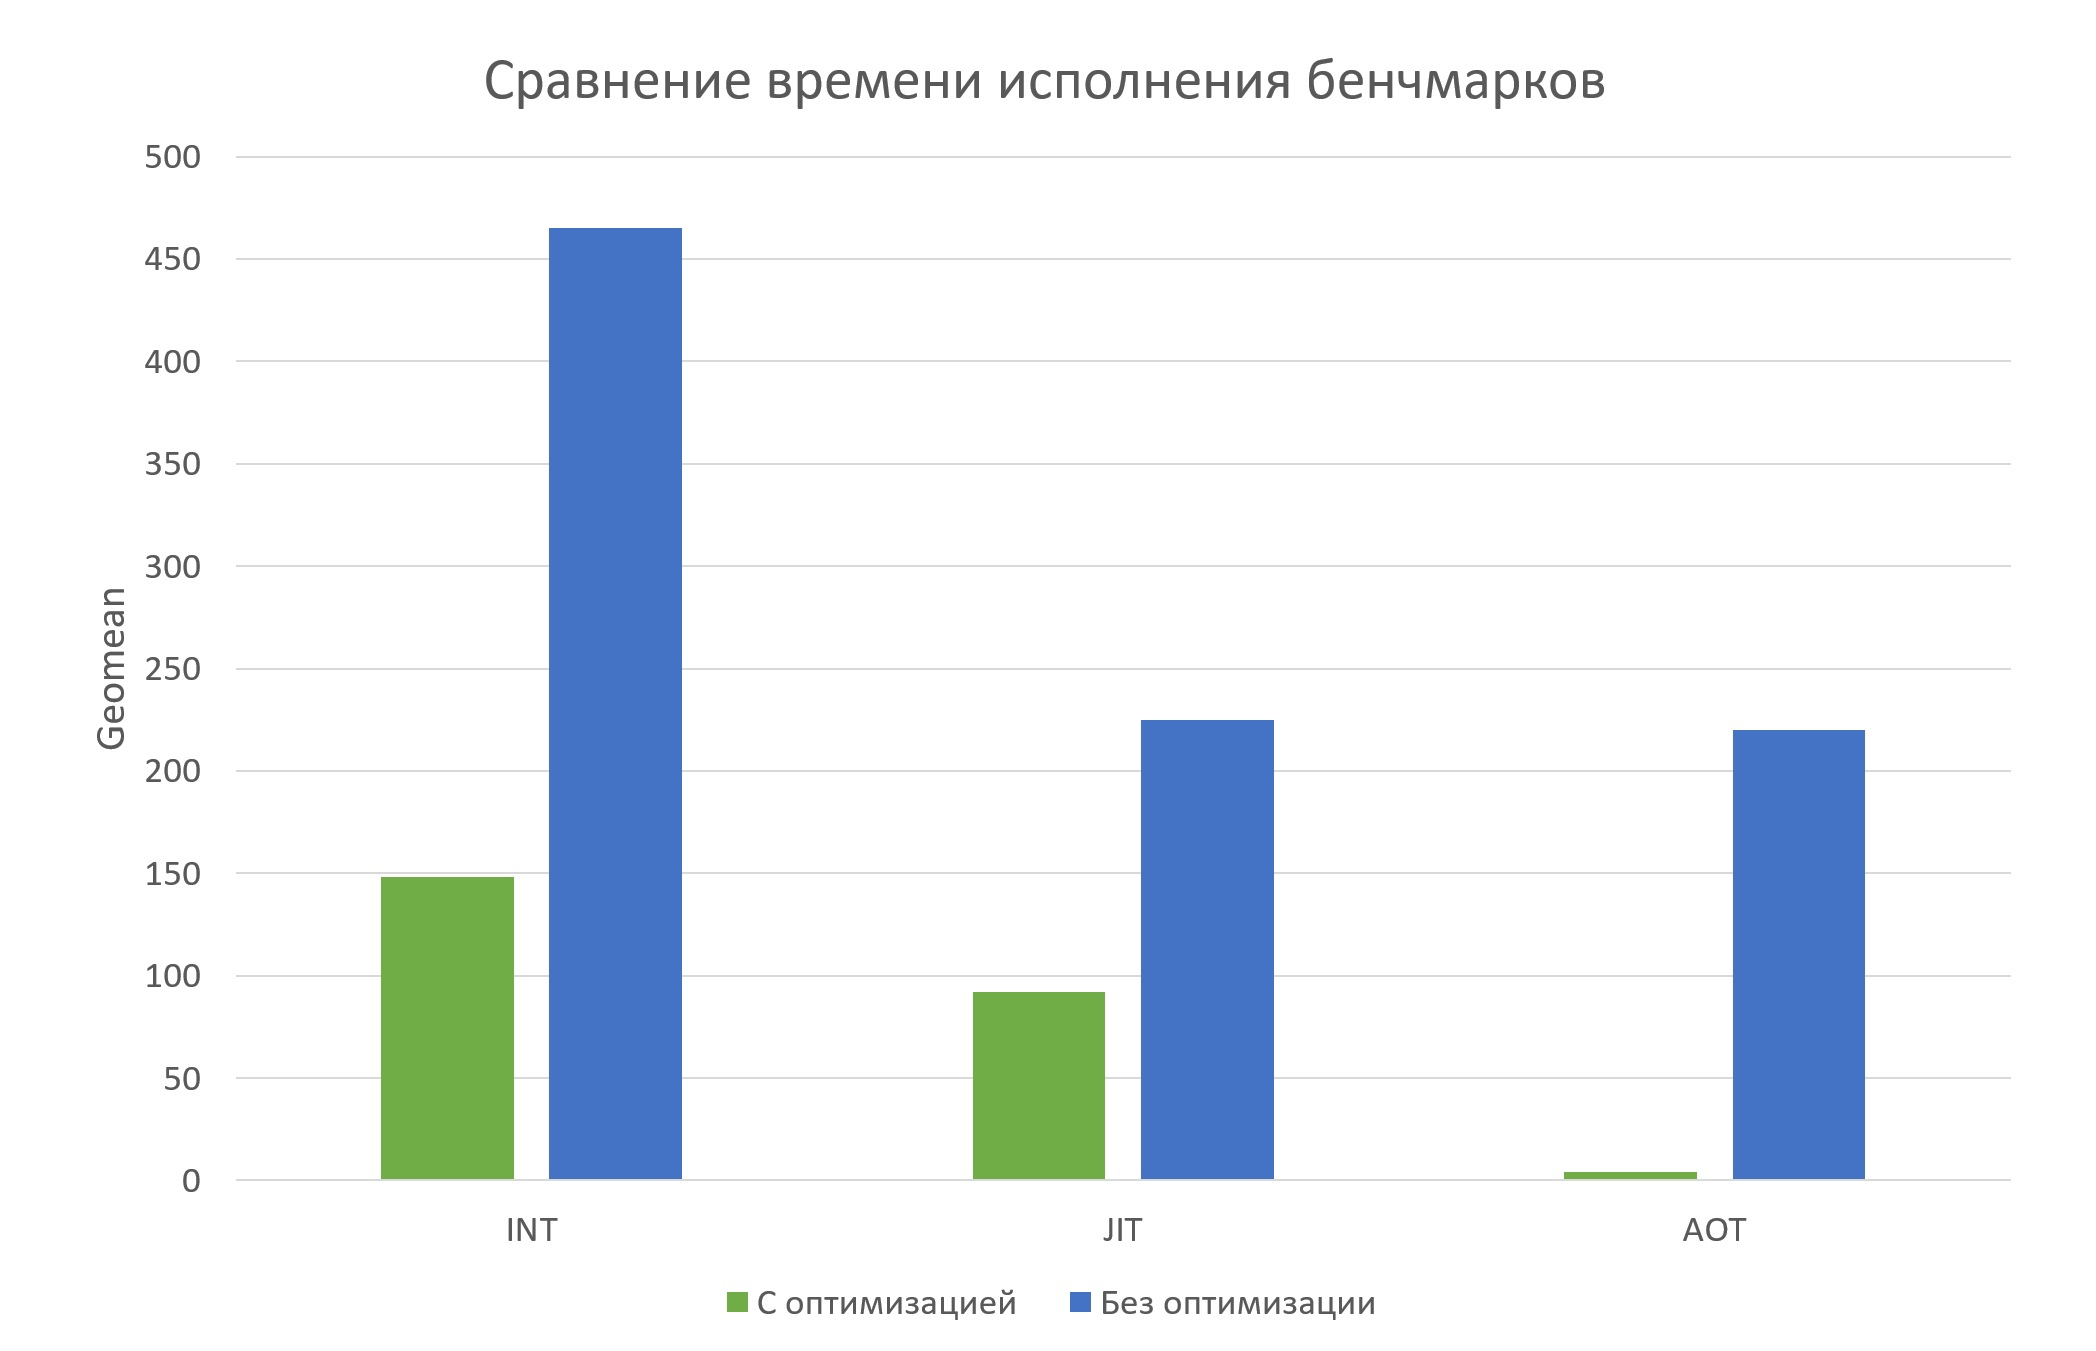
\includegraphics[scale=0.18]{Benches1.jpg}
    \caption{Сравнение времени исполнения бенчмарков}\label{fig:figure}
\end{figure}

Как можно видеть из графиков, увеличение производительности составило:

\begin{itemize}[left=2em]
    \item Для интерпретатора в 3 раза

    \item Для JIT в 2.4 раза

    \item Для AOT в 80 раз
\end{itemize}

Сравнение происходит по геометрическому среднему всех замеров.
Стоит отметить, что бенчмарки не случайные и выбирались специальным образом.
В них широко используются тернарные выражения, порождающие объединения с литеральными типами, причем в огромных циклах.
Также используются функции стандартной библиотеки, в которых также активно задействованы данные операции.
Такой выбор бенчмарков связан с тем, что оптимизация сама по себе является довольно узкоспециализированной, и сравнивать
тесты без числовых объединений не имеет особого смысла.


\newpage
